\documentclass[UTF8]{ctexart} % 添加中文支持

% documentclass到begin之间称为导言区,可以在这里进行一些全局设置

% 使用usepackage来添加宏包
% 所谓宏包,就是一系列控制序列的合集,这些控制序列太常用,以至于人们会觉得每次将他们写在导言区太过繁琐,于是将他们打包放在同一个文件中
% 宏包就是用于拓展Latex功能的
\usepackage{graphicx} % 用于导入外部图片的宏包(推荐格式pdf>>>>png>jpg>eps)
\usepackage{amsmath} % 使用 AMS-LaTeX 提供的数学功能
\usepackage{lmodern} % 解决字体警告问题
% \usepackage[pdf]{graphviz} % graphviz绘图支持(需要安装graphviz)
% 我的评价是还不如把latex和graphviz分开使用(latex渲染,graphviz绘图,不必非得把两者合并到一起)
\usepackage{float} % 防止图片乱浮动导致图片文字顺序混乱的包
\usepackage{multirow} % 多行表格合并的宏包
\usepackage{diagbox} % 表头斜线分割宏包
\usepackage{listings} % 代码块宏包
\usepackage{color} % 颜色宏包
\usepackage{arydshln} % 表格虚线宏包
\usepackage{amssymb} % 数学符号宏包

\lstset{
    basicstyle          =   \ttfamily,          % 基本代码风格
    keywordstyle        =   \bfseries,          % 关键字风格
    commentstyle        =   \rmfamily\itshape,  % 注释的风格,斜体
    stringstyle         =   \ttfamily,  % 字符串风格
    flexiblecolumns,                % 别问为什么,加上这个
    numbers             =   left,   % 行号的位置在左边
    showspaces          =   false,  % 是否显示空格,显示了有点乱,所以不现实了
    numberstyle         =   \zihao{-5}\ttfamily,    % 行号的样式,小五号,tt等宽字体
    showstringspaces    =   false,
    captionpos          =   t,      % 这段代码的名字所呈现的位置,t指的是top上面
    frame               =   lrtb,   % 显示边框
}

\lstdefinestyle{Python}{
    language        =   Python, % 语言选Python
    basicstyle      =   \zihao{-5}\ttfamily,
    numberstyle     =   \zihao{-5}\ttfamily,
    keywordstyle    =   \color{blue},
    keywordstyle    =   [2] \color{teal},
    stringstyle     =   \color{magenta},
    commentstyle    =   \color{red}\ttfamily,
    breaklines      =   true,   % 自动换行,建议不要写太长的行
    columns         =   fixed,  % 如果不加这一句,字间距就不固定,很丑,必须加
    basewidth       =   0.5em,
}

\lstdefinestyle{c}{
    language        =   c, % 语言选Python
    basicstyle      =   \zihao{-5}\ttfamily,
    numberstyle     =   \zihao{-5}\ttfamily,
    keywordstyle    =   \color{blue},
    keywordstyle    =   [2] \color{teal},
    stringstyle     =   \color{magenta},
    commentstyle    =   \color{red}\ttfamily,
    breaklines      =   true,   % 自动换行,建议不要写太长的行
    columns         =   fixed,  % 如果不加这一句,字间距就不固定,很丑,必须加
    basewidth       =   0.5em,
}

\title{编译原理复习}
\author{Garone Lombard}
\date{\today}

\begin{document}

% 根据导言区设置生成标题、作者、日期
\maketitle % Insert the title, author and date

\newpage

\begin{abstract}
    编译原理烤漆复习手册
\end{abstract}

\newpage

% 生成目录(需要注意的是,目录的正确生成至少需要编译两次)
\tableofcontents

\newpage

\section{绪论}

\paragraph{编译程序概念} 用高级语言编制的程序,计算机不能立即执行, 必须通过一个“翻译程序”加工,转化为与其等价的机器语言程序,机器才能执行。这种翻译程序,称之为\textbf{编译程序}

\paragraph{源程序} 用\emph{汇编语言}或\emph{高级语言}编写的程序称为源程序

\paragraph{目标程序} 用\textbf{目标语言}所表示的程序

\paragraph{目标语言} 可以是介于源语言和机器语言之间的“中间语言”,可以是某种机器的机器语言也可以是某机器的汇编语言

\paragraph{翻译程序} 将源程序转换为目标程序的程序称为翻译程序,指各种语言的翻译器,包括汇编程序和编译程序,\emph{是汇编程序、编译程序以及各种变换程序的总称}

\paragraph{汇编} 若源程序用汇编语言书写,经过翻译程序得到用机器语言 表示的程序,这时的翻译程序就称之为汇编程序,这种翻译过程称为汇编

\paragraph{编译} 若源程序是用高级语言书写,经加工后得到目标程序, 这种翻译过程称“编译”(Compile)

\paragraph{编译程序5阶段都要做的事} 符号表管理+错误处理

\paragraph{遍} 遍:对源程序(包括源程序中间形式)从头到尾扫描一次, 并做有关的加工处理 ,生成新的源程序中间形式或目标程序,通常称之为一遍。

\paragraph{生成中间代码的目的} 便于优化处理、便于编译程序的移植

\paragraph{扩充的BNF表示} 就是比BNF多了一些符号,比如$[...]$表示可选项,$\{...\}$表示重复0次或多次,$(...)$表示0次或1次

\section{文法和语言}

\paragraph{文法定义} 四元组
\begin{equation}
    G=(V_T,V_N,P,S)
\end{equation}
\subsection{文法的分类}

\paragraph{0型文法} 无限制文法,只要求\emph{产生式的左部存在一个非终结符}即可。

\begin{equation}
    \forall \alpha \rightarrow \beta \in P \qquad \alpha\text{中至少包含一个}V_N
\end{equation}

\paragraph{1型文法} 上下文有关文法,在\underline{0型文法的基础上}进一步要求\emph{产生式的左部长度小于等于右部长度}
\begin{equation}
    \begin{aligned}
        \forall \alpha \rightarrow \beta \in P \qquad |\alpha| \leq |\beta| \\
        \text{产生式的一般形式}\quad \alpha1A\alpha2 \rightarrow \alpha1\beta\alpha2(\beta \neq \epsilon)
    \end{aligned}
\end{equation}

\paragraph{2型文法} 上下文无关文法(\textbf{可以描述大部分程序设计语言的文法构造}),要求\emph{产生式的左部只能是一个非终结符}

\begin{equation}
    \forall \alpha \rightarrow \beta \in P \qquad \alpha \in V_N
\end{equation}

\paragraph{3型文法} 正则文法,只有两种形式,左线性文法or右线性文法(注意是要求某一文法的所有产生式均符合左/右线性文法,而不只是P1满足左线性,P2满足右线性)。\\
正则文法和正则表达式是等价的,对于任意一个正则文法G,都存在定义同一语言的正则表达式r,反之亦然。

\begin{itemize}
    \item 左线性文法:$A\rightarrow \omega B \quad or \quad A\rightarrow \omega $
    \item 右线性文法:$A\rightarrow B \omega \quad or \quad A\rightarrow \omega $
\end{itemize}

例如
\begin{align*}
    S & \rightarrow a|b|c|d                       \\
    S & \rightarrow aT|bT|cT|dT                   \\
    T & \rightarrow a|b|c|d|0|1|2|3|4|5           \\
    T & \rightarrow aT|bT|cT|dT|0T|1T|2T|3T|4T|5T
\end{align*}

\subsection{(句型的)短语}

已知文法

\begin{align*}
    E & \rightarrow E+E    \\
    E & \rightarrow E*E    \\
    E & \rightarrow -E     \\
    E & \rightarrow (E)    \\
    E & \rightarrow idenfr \\
\end{align*}

对于句型:$-(E+E)$,可构造如下分析树

% 对于图片浮动的问题,还是得手动排版来解决
\begin{figure}[H]
    \centering
    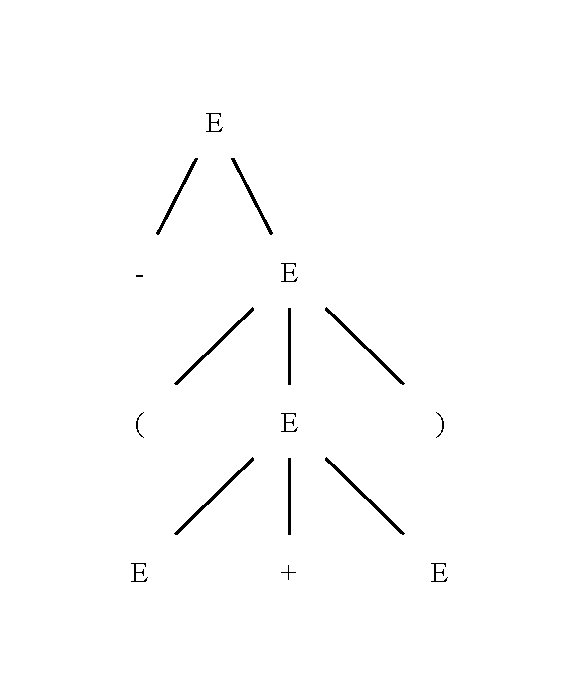
\includegraphics[width=0.7\textwidth]{assets/tree.pdf}
    \caption{分析树}
\end{figure}

\begin{itemize}
    \item $E+E$是句型$-(E+E)$相对于规则$E\rightarrow E+E$的短语,直接短语,句柄(子树层级为1)
    \item $(E+E)$是句型$-(E+E)$相对于规则$E\rightarrow (E)$的短语
    \item $-(E+E)$是句型$-(E+E)$相对于规则$E\rightarrow -E$的短语
\end{itemize}

需要注意的是,直接短语一定是某产生式的右部,但\emph{某产生式的右部不一定是\textbf{给定句型}的直接短语}

\section{词法分析}

\subsection{有穷自动机}

\paragraph{基本概念} 省略...

\begin{figure}[H]
    \centering
    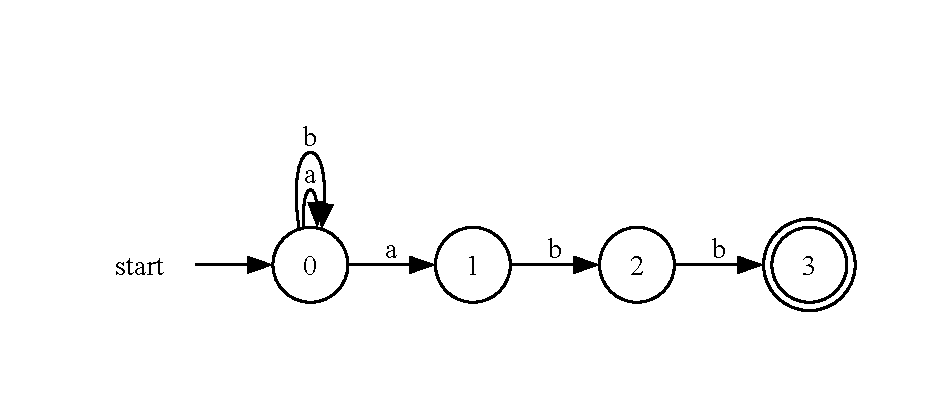
\includegraphics[width=\textwidth]{assets/FA.pdf}
    \caption{FA}
\end{figure}

\paragraph{最长前缀匹配原则} 当输入串的多个前缀与一个或多个模式匹配时,总是选择最长的前缀匹配。
也就是说在到达某个终态后,只要输入串上还有符号,FA就会继续读入下一个符号,以寻求尽可能长度的匹配。

\emph{正则表达式和有穷自动机是等价的}

\subsubsection{确定的有穷自动机(DFA)}

\paragraph{定义} DFA是一个五元组,$M=(S,\Sigma,\delta,s_0,F)$

\begin{itemize}
    \item S:有穷状态集
    \item $\Sigma$:输入符号表
    \item $\delta$:状态转移函数,$\forall s\in S,a\in \Sigma,\delta(s,a)$表示从状态s出发,沿着标记为a的边所能到达的状态(\emph{唯一})
    \item $s_0$:初始状态
    \item F:终态\textbf{集}
\end{itemize}

\begin{figure}[H]
    \centering
    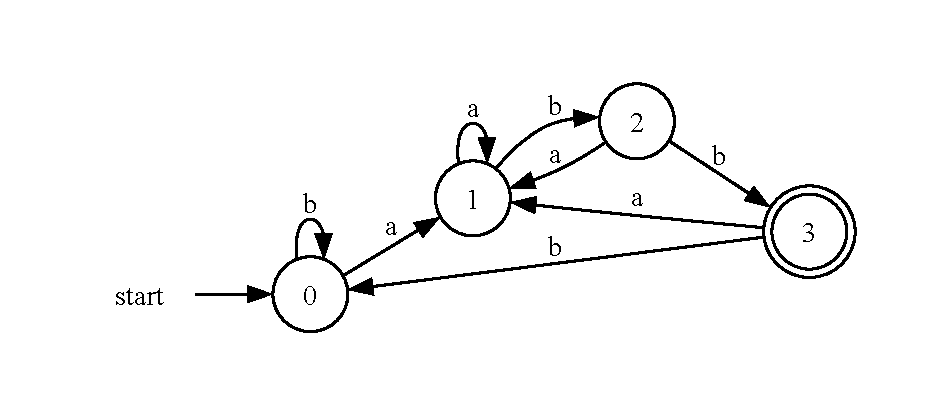
\includegraphics[width=\textwidth]{assets/DFA.pdf}
    \caption{DFA}
\end{figure}

\begin{table}[H]
    \centering
    \begin{tabular}{|p{2cm}<{\centering}|p{3cm}<{\centering}|p{3cm}<{\centering}|}
        \hline
        \diagbox{状态}{输入} & a & b \\
        \hline
        0                & 1 & 0 \\
        \hline
        1                & 1 & 2 \\
        \hline
        2                & 1 & 3 \\
        \hline
        3*               & 1 & 0 \\
        \hline
    \end{tabular}
    \caption{转换表}
\end{table}

\paragraph{DFA的算法实现}

\begin{itemize}
    \item 输入:以文件结束符eof结尾的字符串x,DFA M的开始状态$s_0$,接受状态集合F,状态转换函数$move(s,a)$
    \item 输出:M接受则输出"yes",拒绝则输出"no"
    \item 算法:
          \begin{lstlisting}[language=c,style=c]
s=s0;
c=nextChar();
while(c!=eof){
    s=move(s,c);
    c=nextChar();
}
if(s in F) output("yes");
else output("no");
          \end{lstlisting}
\end{itemize}

\subsubsection{不确定的有穷自动机(NFA)}

\paragraph{定义} NFA是一个五元组,$M=(S,\Sigma,\delta,s_0,F)$

\begin{itemize}
    \item S:有穷状态集
    \item $\Sigma$:输入符号表
    \item $\delta$:状态转移函数,$\forall s\in S,a\in \Sigma,\delta(s,a)$表示从状态s出发,沿着标记为a的边所能到达的状态\textbf{集合}
    \item $s_0$:初始状态
    \item F:终态\textbf{集}
\end{itemize}

\emph{NFA和DFA的唯一区别就是状态转换函数的状态不唯一}

\begin{figure}[H]
    \centering
    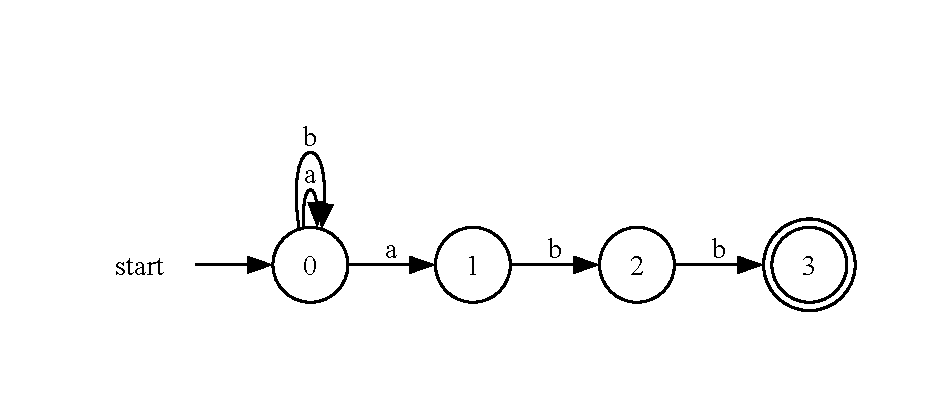
\includegraphics[width=\textwidth]{assets/NFA.pdf}
    \caption{NFA}
\end{figure}

\begin{table}[H]
    \centering
    \begin{tabular}{|p{2cm}<{\centering}|p{3cm}<{\centering}|p{3cm}<{\centering}|}
        \hline
        \diagbox{状态}{输入} & a       & b      \\
        \hline
        0                & \{0,1\} & \{0\}  \\
        \hline
        1                & $\phi$  & \{2\}  \\
        \hline
        2                & $\phi$  & \{3\}  \\
        \hline
        3*               & $\phi$  & $\phi$ \\
        \hline
    \end{tabular}
    \caption{转换表}
\end{table}

\emph{DFA和NFA具有等价性},即对于任意一个NFA,都存在一个DFA,使得两者能够识别相同的语言,反之亦然。

\paragraph{带有$\epsilon$ 转换的NFA} $\epsilon$-NFA,是一种特殊的NFA,其状态转换函数$\delta$中,$\delta(s,\epsilon)$表示从状态s出发,不读入任何输入符号,直接转移到下一个状态。

\begin{figure}[H]
    \centering
    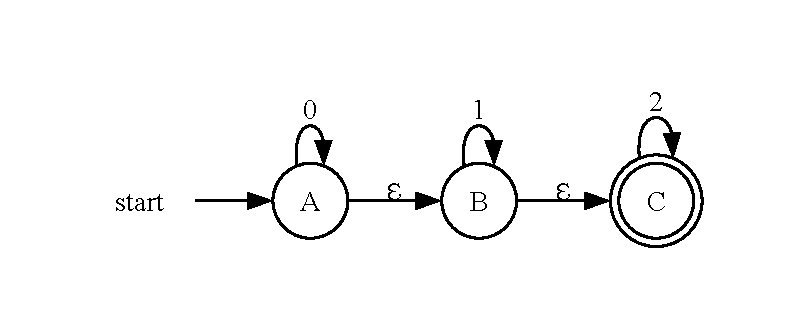
\includegraphics[width=\textwidth]{assets/epsilon-NFA.pdf}
    \caption{$\epsilon$-NFA}
\end{figure}

可以证明,对于任意一个$\epsilon$-NFA,都存在一个DFA,使得两者能够识别相同的语言,反之亦然。

也就是说,\emph{DFA、NFA、$\epsilon$-NFA都具有等价性}。

\subsubsection{从正则表达式到DFA的转换}

直接将正则表达式转换为DFA相当困难,所以一般采取$RE->NFA->DFA$的形式

\paragraph{正则表达式到NFA的转换} 对应关系如下

\begin{itemize}
    \item $\epsilon$对应的NFA
          \begin{figure}[H]
              \centering
              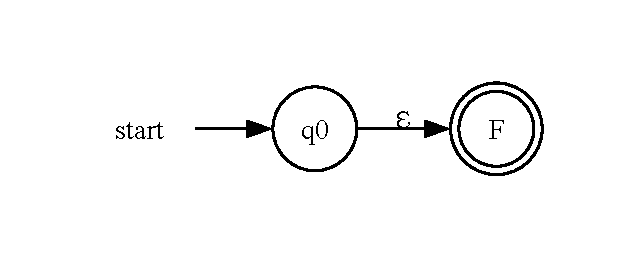
\includegraphics[width=0.7\textwidth]{assets/空串NFA.pdf}
          \end{figure}
    \item 字母表$\Sigma$中符号a对应的NFA
          \begin{figure}[H]
              \centering
              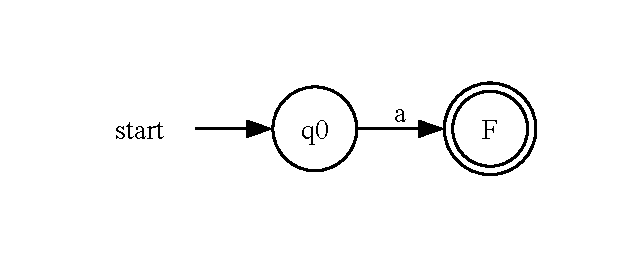
\includegraphics[width=0.7\textwidth]{assets/aNFA.pdf}
          \end{figure}
    \item $r=r_1r_2$对应的NFA
          \begin{figure}[H]
              \centering
              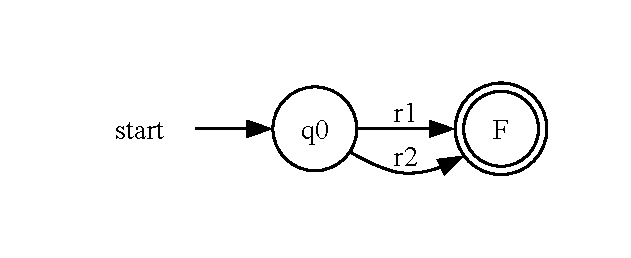
\includegraphics[width=0.7\textwidth]{assets/r1orr2NFA.pdf}
          \end{figure}
    \item $r=(r_1)*$对应的NFA
          \begin{figure}[H]
              \centering
              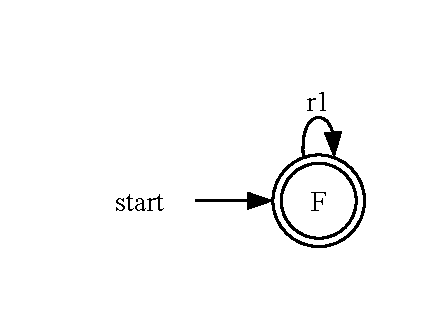
\includegraphics[width=0.7\textwidth]{assets/r1NFA.pdf}
          \end{figure}
    \item $r=(a|b)^*abb$对应的NFA
          \begin{figure}[H]
              \centering
              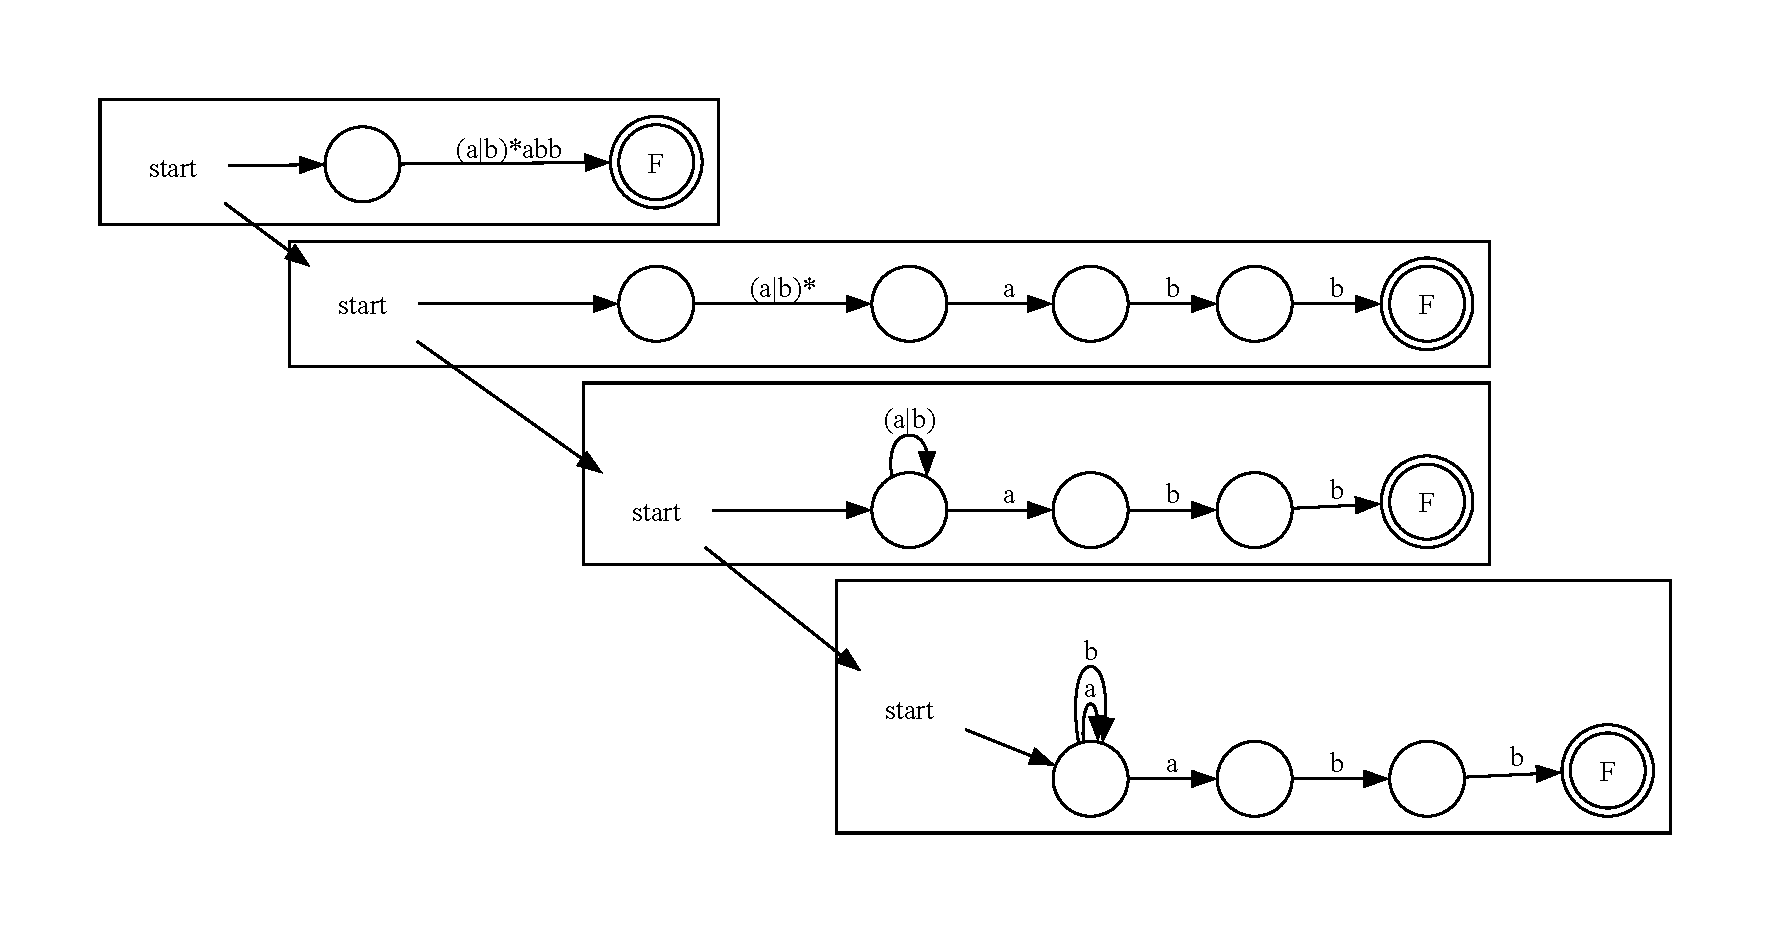
\includegraphics[width=\textwidth]{assets/ababb.pdf}
          \end{figure}
\end{itemize}

\paragraph{NFA到DFA的转换} 如下所示

\begin{figure}[H]
    \centering
    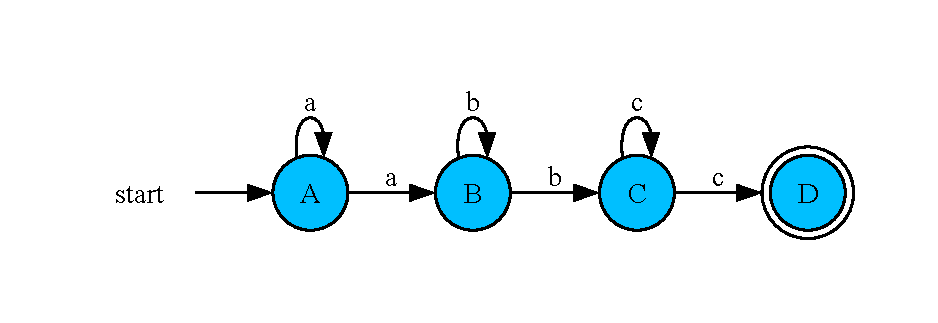
\includegraphics[width=\textwidth]{assets/nfa2.pdf}
\end{figure}

首先绘制状态转换表

\begin{table}[H]
    \centering
    \begin{tabular}{|p{2cm}<{\centering}|p{2cm}<{\centering}|p{2cm}<{\centering}|p{2cm}<{\centering}|}
        \hline
        \diagbox{状态}{输入} & a       & b       & c       \\
        \hline
        A                & \{A,B\} & $\phi$  & $\phi$  \\
        \hline
        B                & $\phi$  & \{B,C\} & $\phi$  \\
        \hline
        C                & $\phi$  & $\phi$  & \{C,D\} \\
        \hline
        D*               & $\phi$  & $\phi$  & $\phi$  \\
        \hline
    \end{tabular}
    \caption{转换表}
\end{table}

与NFA等价的DFA的每一个状态都是一个由NFA状态构成的集合

\begin{figure}[H]
    \centering
    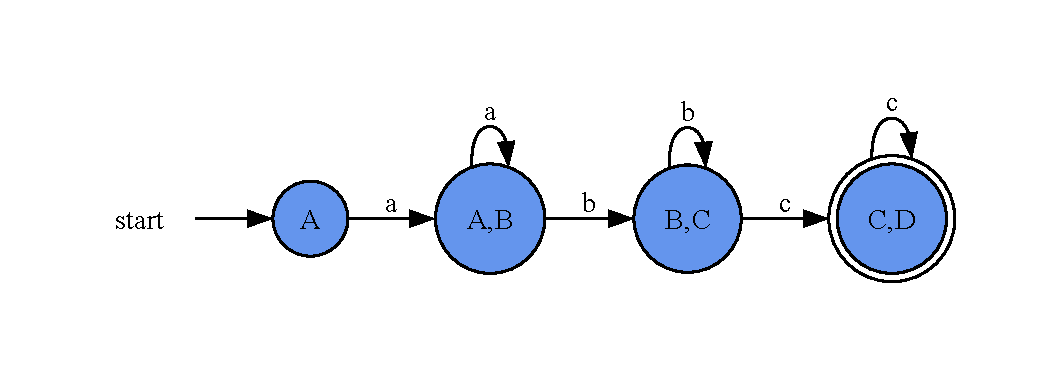
\includegraphics[width=\textwidth]{assets/dfa2.pdf}
\end{figure}

$\epsilon$-NFA到DFA的转换

\begin{figure}[H]
    \centering
    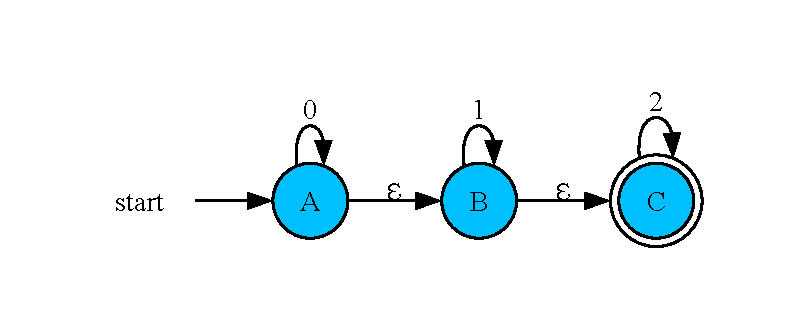
\includegraphics[width=\textwidth]{assets/nfa3.pdf}
\end{figure}

同样绘制状态转换表

\begin{table}[H]
    \centering
    \begin{tabular}{|p{2cm}<{\centering}|p{2cm}<{\centering}|p{2cm}<{\centering}|p{2cm}<{\centering}|}
        \hline
        \diagbox{状态}{输入} & 0         & 1       & 2     \\
        \hline
        A                & \{A,B,C\} & \{B,C\} & \{C\} \\
        \hline
        B                & $\phi$    & \{B,C\} & \{C\} \\
        \hline
        C*               & $\phi$    & $\phi$  & \{C\} \\
        \hline
    \end{tabular}
    \caption{转换表}
\end{table}

需要注意的是,由于初始即可达A,B,C,所以初始状态应该是{A,B,C}而不是{A}

\begin{figure}[H]
    \centering
    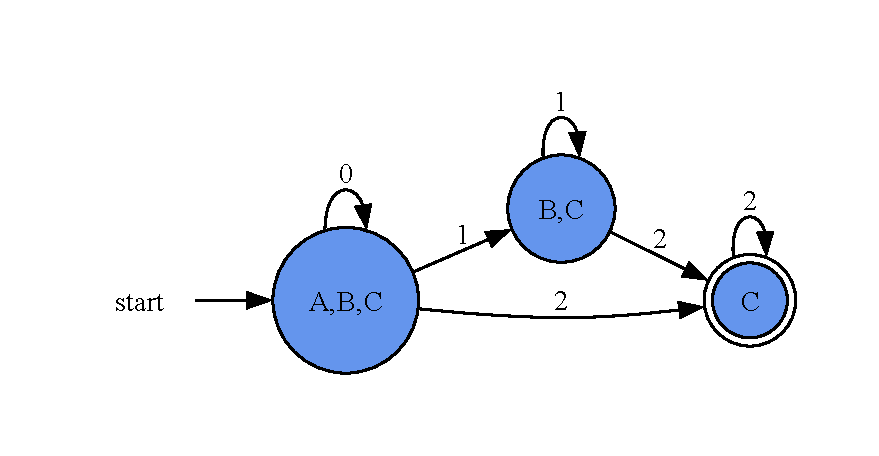
\includegraphics[width=\textwidth]{assets/dfa3.pdf}
\end{figure}

\paragraph{子集构造法}

\begin{itemize}
    \item 输入:NFA N
    \item 输出:DFA D
    \item 算法:一开始,$\epsilon-closure(s_0)$是Dstates中唯一的状态,且未加标记;
          \begin{lstlisting}[language=c,style=c]
while(在Dstates中有一个未标记状态T){
    tag(T);
    for(每个输入符号a){
        U=closure(move(T,a));
        if(U not in Dstates){
            add(Dstates,U);
        }
        Dtran[T,a]=U;
    }
}
          \end{lstlisting}
          \begin{table}[H]
              \centering
              \begin{tabular}{|p{3cm}<{\centering}|p{8cm}<{\centering}|}
                  \hline
                  操作                    & 描述                                        \\
                  \hline
                  $\epsilon-closure(s)$ & 能够从NFA的开始状态只通过$\epsilon$转换直接到达的NFA状态集合    \\
                  \hline
                  $\epsilon-closure(T)$ & 能从集合T中的某个NFA状态只通过$\epsilon$转换直接到达的NFA状态集合 \\
                  \hline
                  $move(T,a)$           & 能从集合T中的某个NFA状态通过标号为a的转换到达的NFA状态的集合        \\
                  \hline
              \end{tabular}
          \end{table}
\end{itemize}

\paragraph{NFA的化简例题} 。。。。。。

\begin{figure}[H]
    \centering
    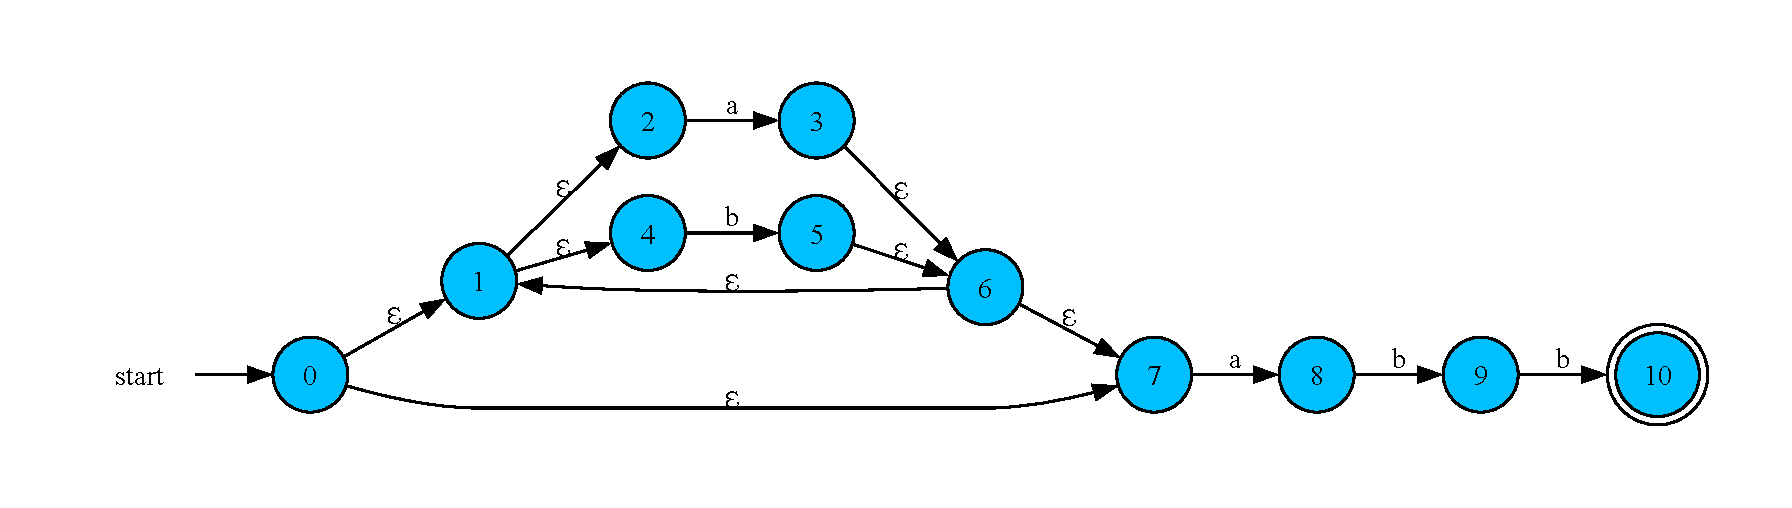
\includegraphics[width=\textwidth]{assets/nfa4.pdf}
    \caption{NFA}
\end{figure}

\begin{table}[H]
    \centering
    \begin{tabular}{|p{2cm}<{\centering}|p{3cm}<{\centering}|p{3cm}<{\centering}|}
        \hline
        \diagbox{状态}{输入} & a                 & b               \\
        \hline
        0                & \{1,2,3,4,6,7,8\} & \{1,2,4,5,6,7\} \\
        \hline
        1                & \{1,2,3,4,6,7\}   & \{1,2,4,5,6,7\} \\
        \hline
        2                & \{1,2,3,4,6,7\}   & $\phi$          \\
        \hline
        3                & \{1,2,3,4,6,7,8\} & \{1,2,4,5,6,7\} \\
        \hline
        4                & $\phi$            & \{1,2,4,5,6,7\} \\
        \hline
        5                & \{1,2,3,4,6,7,8\} & \{1,2,4,5,6,7\} \\
        \hline
        6                & \{1,2,3,4,6,7,8\} & \{1,2,4,5,6,7\} \\
        \hline
        7                & \{8\}             & $\phi$          \\
        \hline
        8                & $\phi$            & \{9\}           \\
        \hline
        9                & $\phi$            & \{10\}          \\
        \hline
        10*              & $\phi$            & $\phi$          \\
        \hline
    \end{tabular}
    \caption{转换表1(无效)}
\end{table}

\begin{table}[H]
    \centering
    \begin{tabular}{|p{3.2cm}<{\centering}|p{3cm}<{\centering}|p{3cm}<{\centering}|}
        \hline
        $\epsilon-closure(T_0)$ & \multicolumn{2}{c|}{\{0,1,2,4,7\}}                      \\
        \hline
        \diagbox{状态}{输入}        & a                                  & b                  \\
        \hline
        T0=\{0,1,2,4,7\}        & \{1,2,3,4,6,7,8\}                  & \{1,2,4,5,6,7\}    \\
        \hline
        T1=\{1,2,3,4,6,7,8\}    & \{1,2,3,4,6,7,8\}                  & \{1,2,4,5,6,7,9\}  \\
        \hline
        T2=\{1,2,4,5,6,7\}      & \{1,2,3,4,6,7,8\}                  & \{1,2,4,5,6,7\}    \\
        \hline
        T3=\{1,2,4,5,6,7,9\}    & \{1,2,3,4,6,7,8\}                  & \{1,2,4,5,6,7,10\} \\
        \hline
        T4=\{1,2,4,5,6,7,10\}   & \{1,2,3,4,6,7,8\}                  & \{1,2,4,5,6,7\}    \\
        \hline
    \end{tabular}
    \caption{转换表2(正确)}
\end{table}

\begin{table}[H]
    \centering
    \begin{tabular}{|p{3.4cm}<{\centering}|p{3cm}<{\centering}|p{3cm}<{\centering}|}
        \hline
        \diagbox{状态}{输入}       & a  & b  \\
        \hline
        T0=\{0,1,2,4,7\}       & T1 & T2 \\
        \hline
        T1=\{1,2,3,4,6,7,8\}   & T1 & T3 \\
        \hline
        T2=\{1,2,4,5,6,7\}     & T1 & T2 \\
        \hline
        T3=\{1,2,4,5,6,7,9\}   & T1 & T4 \\
        \hline
        T4*=\{1,2,4,5,6,7,10\} & T1 & T2 \\
        \hline
    \end{tabular}
    \caption{转换表2(正确)}
\end{table}

\begin{figure}[H]
    \centering
    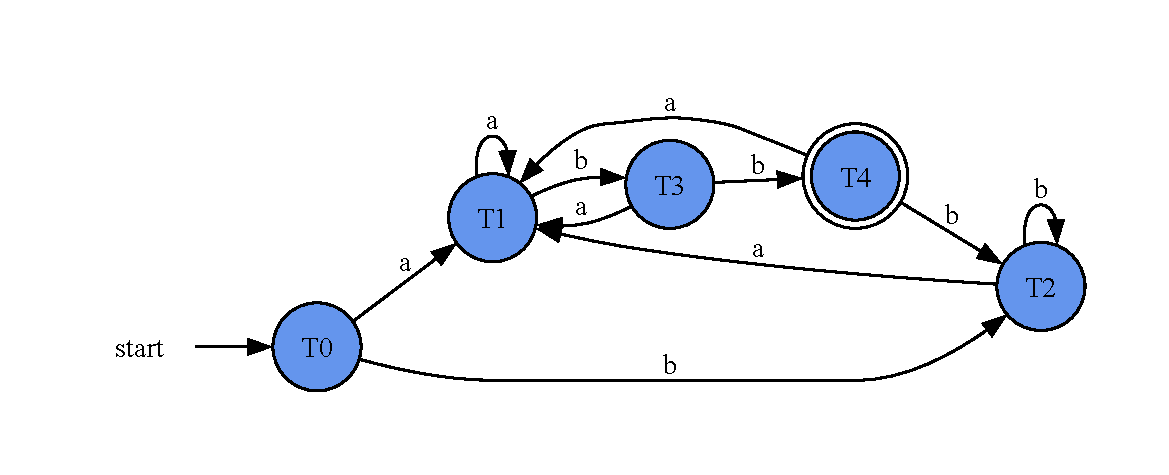
\includegraphics[width=\textwidth]{assets/dfa4.pdf}
    \caption{DFA}
\end{figure}

\subsubsection{DFA的最小化}

\paragraph{概念} 一个有穷自动机可以通过\emph{消除无用状态}和\emph{合并等价状态}来最小化

\begin{itemize}
    \item 无用状态:从该自动机的开始状态出发,任何输入串都无法到达的状态(从该状态出发,没有通路抵达终态)
    \item 等价状态:条件如下
          \begin{enumerate}
              \item \underline{一致性条件}:状态s和t必须同时为可接受状态或不可接受状态
              \item \underline{蔓延性条件}:对于所有输入符号,状态s和t必须转换到等价态
          \end{enumerate}
\end{itemize}

\paragraph{分割法} 把一个DFA(不含无用态)的状态分成一些不相交的子集,使得任何不同的两个子集的状态都是可区分的,且同一个子集中的任何状态都是等价的

\begin{figure}[H]
    \centering
    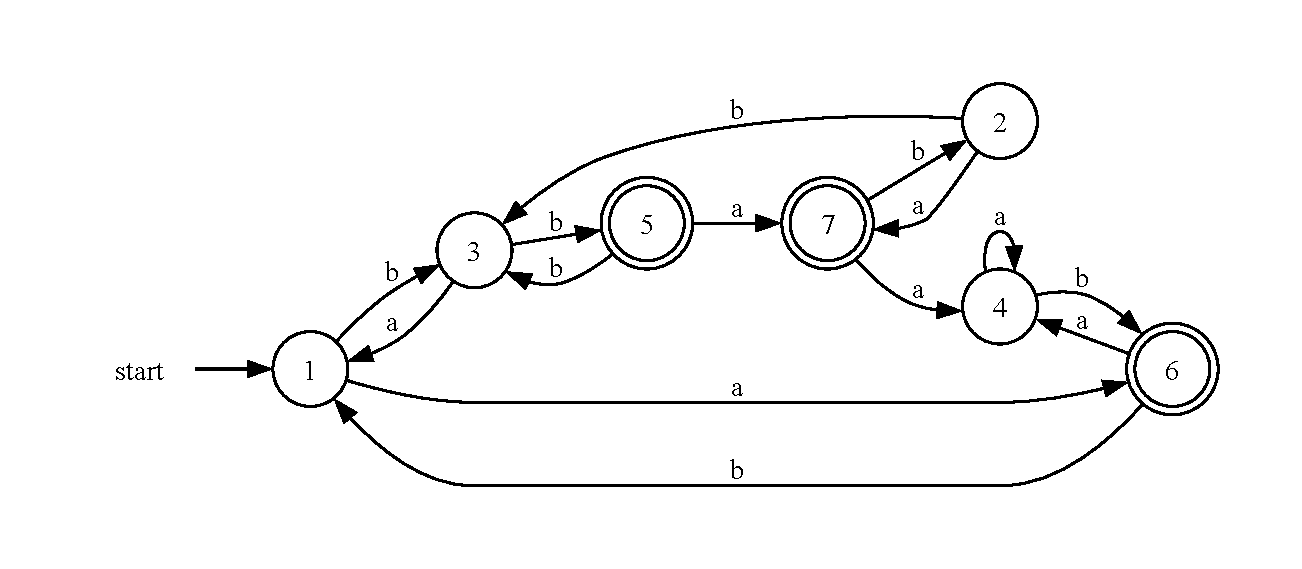
\includegraphics[width=\textwidth]{assets/dfa5.pdf}
\end{figure}

第一步都是固定的,把状态分为终态和非终态两个集合\{1,2,3,4\},\{5,6,7\}

接下来考察\{1,2,3,4\}是否可分

\begin{table}[H]
    \centering
    \begin{tabular}{|p{3cm}<{\centering}|p{2cm}<{\centering}|p{2cm}<{\centering}|}
        \hline
        \diagbox{状态}{输入} & a     & b     \\
        \hline
        1                & 6(E)  & 3(NE) \\
        \hline
        2                & 7(E)  & 3(NE) \\
        \hdashline
        3                & 1(NE) & 5(E)  \\
        \hline
        4                & 4(NE) & 6(E)  \\
        \hline
    \end{tabular}
\end{table}

因此可以将集合拆分为\{1,2\},\{3,4\},\{5,6,7\}

\begin{table}[H]
    \centering
    \begin{tabular}{|p{3cm}<{\centering}|p{2cm}<{\centering}|p{2cm}<{\centering}|}
        \hline
        \diagbox{状态}{输入} & a     & b     \\
        \hline
        1                & 6(P3) & 3(P2) \\
        \hline
        2                & 7(P3) & 3(P2) \\
        \hline
    \end{tabular}
\end{table}

显然\{1,2\}不可拆分

\begin{table}[H]
    \centering
    \begin{tabular}{|p{3cm}<{\centering}|p{2cm}<{\centering}|p{2cm}<{\centering}|}
        \hline
        \diagbox{状态}{输入} & a     & b     \\
        \hline
        3                & 1(P1) & 5(P3) \\
        \hdashline
        4                & 4(P2) & 6(P3) \\
        \hline
    \end{tabular}
\end{table}

\{3,4\}可拆分为\{3\},\{4\}

此时集合为\{1,2\},\{3\},\{4\},\{5,6,7\}

\begin{table}[H]
    \centering
    \begin{tabular}{|p{3cm}<{\centering}|p{2cm}<{\centering}|p{2cm}<{\centering}|}
        \hline
        \diagbox{状态}{输入} & a     & b     \\
        \hline
        5                & 7(P4) & 3(P2) \\
        \hdashline
        6                & 4(P3) & 1(P1) \\
        \hline
        7                & 4(P3) & 2(P1) \\
        \hline
    \end{tabular}
\end{table}

\{5,6,7\}可拆分为\{5\},\{6,7\}

因此最终得到的集合为\{1,2\},\{3\},\{4\},\{5\},\{6,7\}

\begin{table}[H]
    \centering
    \begin{tabular}{|p{3cm}<{\centering}|p{2cm}<{\centering}|p{2cm}<{\centering}|}
        \hline
        \diagbox{状态}{输入} & a     & b     \\
        \hline
        1                & 6(P5) & 3(P2) \\
        \hline
        2                & 7(P5) & 3(P2) \\
        \hdashline
        3                & 1(P1) & 5(P4) \\
        \hdashline
        4                & 4(P3) & 6(P5) \\
        \hdashline
        5                & 7(P5) & 3(P2) \\
        \hdashline
        6                & 4(P3) & 1(P1) \\
        \hline
        7                & 4(P3) & 2(P1) \\
        \hline
    \end{tabular}
\end{table}

\begin{figure}[H]
    \centering
    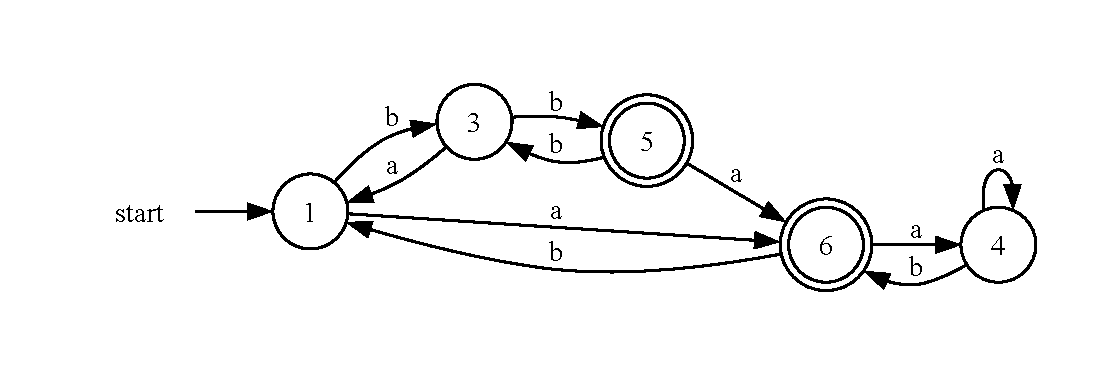
\includegraphics[width=\textwidth]{assets/dfa6.pdf}
    \caption{最小化后的DFA}
\end{figure}

\section{语法分析}

\subsection{自顶向下语法分析}

\paragraph{概念} 从分析树的顶部向底部方向构造分析树,也就是从文法开始符号S从左向右推导句子w的过程

\paragraph{最左推导} 总是选择每个句型的最左非终结符进行替换,其反过程称为最右规约

\paragraph{最右推导} 总是选择每个句型的最右非终结符进行替换,其反过程称为最左规约

在\emph{自底向上的分析}中,总是采用最左规约的方式,因此\textbf{把最左规约成为规范规约},而\textbf{把最右推导称为规范推导}

最左推导和最右推导具备唯一性,因为对于每个句型而言,其最左/右终结符是唯一的

\subsection{文法转换}

\paragraph{左递归文法} 如果一个文法中有一个非终结符A使得对某个串存在推导$A\rightarrow^{+} Aa$,那么这个文法就是左递归文法,这会使递归下降分析器陷入无限循环

处理办法如下(可消除直接左递归,其实是将其转化为了右递归)

\begin{equation}
    \begin{aligned}
        A     & \rightarrow A\alpha|\beta              \\
        A     & \rightarrow A\alpha
        \rightarrow A\alpha\alpha\alpha\alpha
        \rightarrow \beta\alpha\alpha\alpha\alpha\dots \\
        regex & =\beta\alpha^*                         \\
        A     & \rightarrow \beta A^{'}                \\
        A^{'} & \rightarrow \alpha A^{'}|\epsilon
    \end{aligned}
\end{equation}

同理,对于左递归推导$E\rightarrow E+T|T$,消除左递归可得一下等价文法

\begin{equation}
    \begin{aligned}
        E     & \rightarrow TE^{'}           \\
        E^{'} & \rightarrow +TE^{'}|\epsilon
    \end{aligned}
\end{equation}

\paragraph{$\epsilon$产生式的使用时机} 如果当前某终结符A与当前输入a不匹配时,若存在$A\rightarrow\epsilon$,可以通过检查a是否可以出现在A的后面(那不就是查看A的FOLLOW集吗?),来决定是否可以使用产生式$A\rightarrow\epsilon$

\subsubsection{FIRST集}

\paragraph{概念} 串首终结符,给定一个文法符号串a,a的FIRST(a)被定义为可以从a推导出的所有串首终结符的集合,如果$a\Rightarrow^* \epsilon$,那么$\epsilon$也在FIRST(a)中

\subsubsection{FOLLOW集}

\paragraph{概念} 可能在某个句型中紧跟在A后边的终结符a的集合

如果A是某个句型的最右符号,则将结束符\#添加到FOLLOW(A)中

\begin{equation}
    \begin{aligned}
        E     & \rightarrow TE^{'}           \\
        E^{'} & \rightarrow +TE^{'}|\epsilon \\
        T     & \rightarrow FT^{'}           \\
        T^{'} & \rightarrow *FT^{'}|\epsilon \\
        F     & \rightarrow (E)|id
    \end{aligned}
\end{equation}

\begin{equation}
    \begin{aligned}
        FIRST(E)     & = \{(,id\}       \\
        FIRST(E^{'}) & = \{+,\epsilon\} \\
        FIRST(T)     & = \{(,id\}       \\
        FIRST(T^{'}) & = \{*,\epsilon\} \\
        FIRST(F)     & = \{(,id\}
    \end{aligned}
\end{equation}

\begin{equation}
    \begin{aligned}
        FOLLOW(E)     & = \{),\#\}     \\
        FOLLOW(E^{'}) & = \{),\#\}     \\
        FOLLOW(T)     & = \{+,),\#\}   \\
        FOLLOW(T^{'}) & = \{+,),\#\}   \\
        FOLLOW(F)     & = \{*,+,),\#\}
    \end{aligned}
\end{equation}

\begin{equation}
    \begin{aligned}
        E     & \rightarrow TE^{'}           & SELECT(1)=FIRST(T)=\{(,id\}        \\
        E^{'} & \rightarrow +TE^{'}|\epsilon & SELECT(2)=\{+\}                    \\
        E^{'} & \rightarrow \epsilon         & SELECT(3)=FOLLOW(E^{'})=\{),\#\}   \\
        T     & \rightarrow FT^{'}           & SELECT(4)=FIRST(F)=\{(,id\}        \\
        T^{'} & \rightarrow *FT^{'}|\epsilon & SELECT(5)=\{*\}                    \\
        T^{'} & \rightarrow \epsilon         & SELECT(6)=FOLLOW(T^{'})=\{+,),\#\} \\
        F     & \rightarrow (E)|id           & SELECT(7)=\{(\}                    \\
        F     & \rightarrow id               & SELECT(8)=\{id\}
    \end{aligned}
\end{equation}

\subsubsection{SELECT集}

\paragraph{概念} 产生式$A\rightarrow \beta$的可选集是指可以选用该产生式进行推导时对应的输入符号的集合,记为$SELECT(A\rightarrow \beta)$

\begin{itemize}
    \item $SELECT(A\rightarrow \alpha\beta)=\{\alpha\}$
    \item $SELECT(A\rightarrow \epsilon)=FOLLOW(A)$
\end{itemize}

如果每个具有\emph{相同左部}的各个产生式的可选集互不相交的话,就可以做出确定的分析

产生式$A\rightarrow \alpha$的可选集SELECT

\begin{itemize}
    \item 如果$\epsilon \notin FIRST(\alpha)$,则$SELECT(A\rightarrow\alpha)=FIRST(\alpha)$
    \item 如果$\epsilon \in FIRST(\alpha)$,则$SELECT(A\rightarrow\alpha)=(FIRST(\alpha)-\{\epsilon\})\cup FOLLOW(\alpha)$
\end{itemize}

\subsubsection{LL(1)文法}

\paragraph{概念} 文法G是LL(1)的,当且仅当G的任意两个具有相同左部的产生式$A\rightarrow \alpha|\beta$满足下列条件

\begin{itemize}
    \item 如果$\alpha$和$\beta$均不能推导出$\epsilon$,则$FIRST(\alpha)\cap FIRST(\beta)=\phi $
    \item $\alpha$和$\beta$至多只能有一个能推导出$\epsilon$(不能两个均能推导出$\epsilon$,那样的话$SELECT(\alpha)\cap SELECT(\beta)=FOLLOW(A)$,也就是说SELECT集相交了)
          \begin{enumerate}
              \item 如果$\alpha\Rightarrow^* \epsilon$,则$FIRST(\alpha)\cap FOLLOW(A)=\phi$
              \item 如果$\beta\Rightarrow^* \epsilon$,则$FIRST(\beta)\cap FOLLOW(A)=\phi$
          \end{enumerate}
\end{itemize}

总结一句话,就是$SELECT$集别相交就行

\subsection{自底向上语法分析}

\paragraph{概念} 自底向上的语法分析采用最左规约的方式

通用框架:\textbf{移入-归约分析}

\begin{equation}
    \begin{aligned}
        E\rightarrow E+E \\
        E\rightarrow E*E \\
        E\rightarrow (E) \\
        E\rightarrow id
    \end{aligned}
\end{equation}

\begin{table}[H]
    \centering
    \begin{tabular}{|p{3cm}<{\centering}|p{3cm}<{\centering}|p{3cm}<{\centering}|}
        \hline
        栈          & 剩余输入         & 动作                    \\
        \#         & id+(id+id)\# &                       \\
        \# id      & +(id+id)\#   & 移入                    \\
        \# E       & +(id+id)\#   & 归约:$E\rightarrow id$  \\
        \# E+      & (id+id)\#    & 移入                    \\
        \# E+(     & id+id)\#     & 移入                    \\
        \# E+(id   & +id)\#       & 移入                    \\
        \# E+(E    & +id)\#       & 归约:$E\rightarrow id$  \\
        \# E+(E+   & id)\#        & 移入                    \\
        \# E+(E+id & )\#          & 移入                    \\
        \# E+(E+E  & )\#          & 归约:$E\rightarrow id$  \\
        \# E+(E    & )\#          & 归约:$E\rightarrow E+E$ \\
        \# E+(E)   & \#           & 移入                    \\
        \# E+E     & \#           & 归约:$E\rightarrow (E)$ \\
        \# E       & \#           & 归约:$E\rightarrow E+E$ \\
        \hline
    \end{tabular}
\end{table}

\paragraph{移入-归约分析中存在的问题} 句柄的错误识别问题,需要使用LR分析法解决

\begin{equation}
    \begin{aligned}
        <S>\rightarrow var<IDS>:<T> \\
        <IDS>\rightarrow i          \\
        <IDS>\rightarrow <IDS>,i    \\
        <T>\rightarrow real|int
    \end{aligned}
\end{equation}

\begin{table}[H]
    \centering
    \begin{tabular}{|p{5cm}<{\centering}|p{2.4cm}<{\centering}|p{3.4cm}<{\centering}|}
        \hline
        栈                       & 剩余输入             & 动作                          \\
        \#                      & var ia,ib:real\# &                             \\
        \# var                  & ia,ib:real\#     & 移入                          \\
        \# var ia               & ,ib:real\#       & 移入                          \\
        \# var <IDS>            & ,ib:real\#       & 归约:$<IDS>\rightarrow i$     \\
        \# var <IDS>,           & ib:real\#        & 移入                          \\
        \# var <IDS>,ib         & :real\#          & 移入                          \\
        \# var <IDS>,<IDS>      & :real\#          & 归约:$<IDS>\rightarrow i$     \\
        \# var <IDS>,<IDS>:     & real\#           & 移入                          \\
        \# var <IDS>,<IDS>:real & \#               & 移入                          \\
        \# var <IDS>,<IDS>:<T>  & \#               & 归约:$T>\rightarrow real|int$ \\
        \# var <IDS>,<IDS>:<T>  & \#               & ERROR                       \\
        \hline
    \end{tabular}
\end{table}

\subsubsection{LR分析法}

关键问题在于如何\textbf{正确的识别句柄}

\begin{equation}
    \begin{aligned}
        S\rightarrow BB
        B\rightarrow aB
        B\rightarrow b
    \end{aligned}
\end{equation}

\begin{itemize}
    \item sn:将符号a、状态n压入栈
    \item rn:使用第n个产生式进行规约
\end{itemize}

\begin{table}[H]
    \centering
    \begin{tabular}{|p{2cm}<{\centering}|p{1cm}<{\centering}|p{1cm}<{\centering}|p{1cm}<{\centering}|p{1cm}<{\centering}|p{1cm}<{\centering}|p{1cm}<{\centering}|p{1cm}<{\centering}|}
        \hline
        \multirow{2}{*}{状态} & \multicolumn{3}{c|}{ACTION} & \multicolumn{2}{c|}{GOTO}                \\
        \cline{2-6}
        ~                   & a                           & b                         & \#   & S & B \\
        \hline
        0                   & s3                          & s4                        &      & 1 & 2 \\
        \hline
        1                   & ~                           & ~                         & acpt & ~ & ~ \\
        \hline
        2                   & s3                          & s4                        & ~    & ~ & 5 \\
        \hline
        3                   & s3                          & s4                        & ~    & ~ & 6 \\
        \hline
        4                   & r3                          & r3                        & r3   & ~ & ~ \\
        \hline
        5                   & r1                          & r1                        & r1   & ~ & ~ \\
        \hline
        6                   & r2                          & r2                        & r2   & ~ & ~ \\
        \hline
    \end{tabular}
\end{table}

\begin{table}[H]
    \centering
    \begin{tabular}{|p{2cm}<{\centering}|p{2cm}<{\centering}|p{2.4cm}<{\centering}|p{3.4cm}<{\centering}|}
        \hline
        \multicolumn{2}{|c|}{栈} & \multirow{2}{*}{剩余输入} & \multirow{2}{*}{动作}   \\
        \cline{1-2}
        状态                      & 符号                    &                     & \\
        0                       & \#                    & bab\#               & \\
        0 4                     & \# b                  & ab\#                & \\
        0                       & \# B                  & ab\#                & \\
        0 2                     & \# B                  & ab\#                & \\
        0 2 3                   & \# Ba                 & b\#                 & \\
        0 2 3 4                 & \# Bab                & \#                  & \\
        0 2 3                   & \# BaB                & \#                  & \\
        0 2 3 6                 & \# BaB                & \#                  & \\
        0 2                     & \# BB                 & \#                  & \\
        0 2 5                   & \# BB                 & \#                  & \\
        0                       & \# S                  & \#                  & \\
        0 1                     & \# S                  & \#                  & \\
        \hline
    \end{tabular}
\end{table}

\begin{lstlisting}[language=c,style=c]
// 输入符号串为w#,状态栈初始为0
// s代表栈顶状态
while(1){
    if(ACTION[s,a]==st){
        push_state(t);
        push_symbol(a);
    }
    else if(ACTION[s,a]=rt){// rt是归约A->b
        for(int i=0;i<|b|;i++){
            pop_state();
        }
        push_state(GOTO(A,t));
        push_symbol(A);
        output(A->b);
    }
    else if(ACTION[s,a]=accept){
        break;// 语法分析完成
    }
    else{
        ERROR();
    }
}
\end{lstlisting}

LR分析的分析程序非常简单,关键是怎么构造给定文法的LR分析表

\subsubsection{LR(0)分析法}

\paragraph{LR(0)项目的概念} 右部某位置标有原点的产生式称为相应文法的一个LR(0)项目

\begin{equation}
    \begin{aligned}
        A\rightarrow \alpha_1\cdot \alpha_2
    \end{aligned}
\end{equation}

\emph{项目描述了句柄识别的状态}

对于推导$S\rightarrow bBB$

\begin{itemize}
    \item $S\rightarrow \cdot bBB$点右侧是终结符,称为\textbf{移进项目}
    \item $S\rightarrow b\cdot BB$点右侧是非终结符,称为\textbf{待约项目}
    \item $S\rightarrow bB\cdot B$点右侧是非终结符,称为\textbf{待约项目}
    \item $S\rightarrow bBB\cdot$点位于产生式末尾,称为\textbf{归约项目}
    \item $A\rightarrow \epsilon$只对应一个项目$A\rightarrow \cdot$
\end{itemize}

\paragraph{增广文法} 如果G是一个以S为开始符号的文法,则G的增广文法$G^{'}$就是在G中加上新开始符号$S^{'}$和产生式$S^{'}\rightarrow S$而得到的文法

\begin{equation}
    \begin{aligned}
        E & \rightarrow E+T \\
        E & \rightarrow T   \\
        T & \rightarrow T*F \\
        T & \rightarrow F   \\
        F & \rightarrow (E) \\
        F & \rightarrow id
    \end{aligned}
\end{equation}

等价增广文法如下,引入这个新的开始产生式的目的是使得文法开始符号仅出现在一个产生式的左部,从而使得分析器只有一个接受状态

\begin{equation}
    \begin{aligned}
        E^{'} & \rightarrow E   \\
        E     & \rightarrow E+T \\
        E     & \rightarrow T   \\
        T     & \rightarrow T*F \\
        T     & \rightarrow F   \\
        F     & \rightarrow (E) \\
        F     & \rightarrow id
    \end{aligned}
\end{equation}

\paragraph{后继项目} 同属于一个产生式的项目,但圆点的位置只相差一个符号,则称后者是前者的后继项目

比如$S\rightarrow \alpha b\cdot \beta$就是$S\rightarrow \alpha \cdot b \beta$的后继项目

可以把所有等价的项目组成一个项目集,称为项目集闭包,每个项目集闭包对应着自动机的一个状态

\begin{figure}[H]
    \centering
    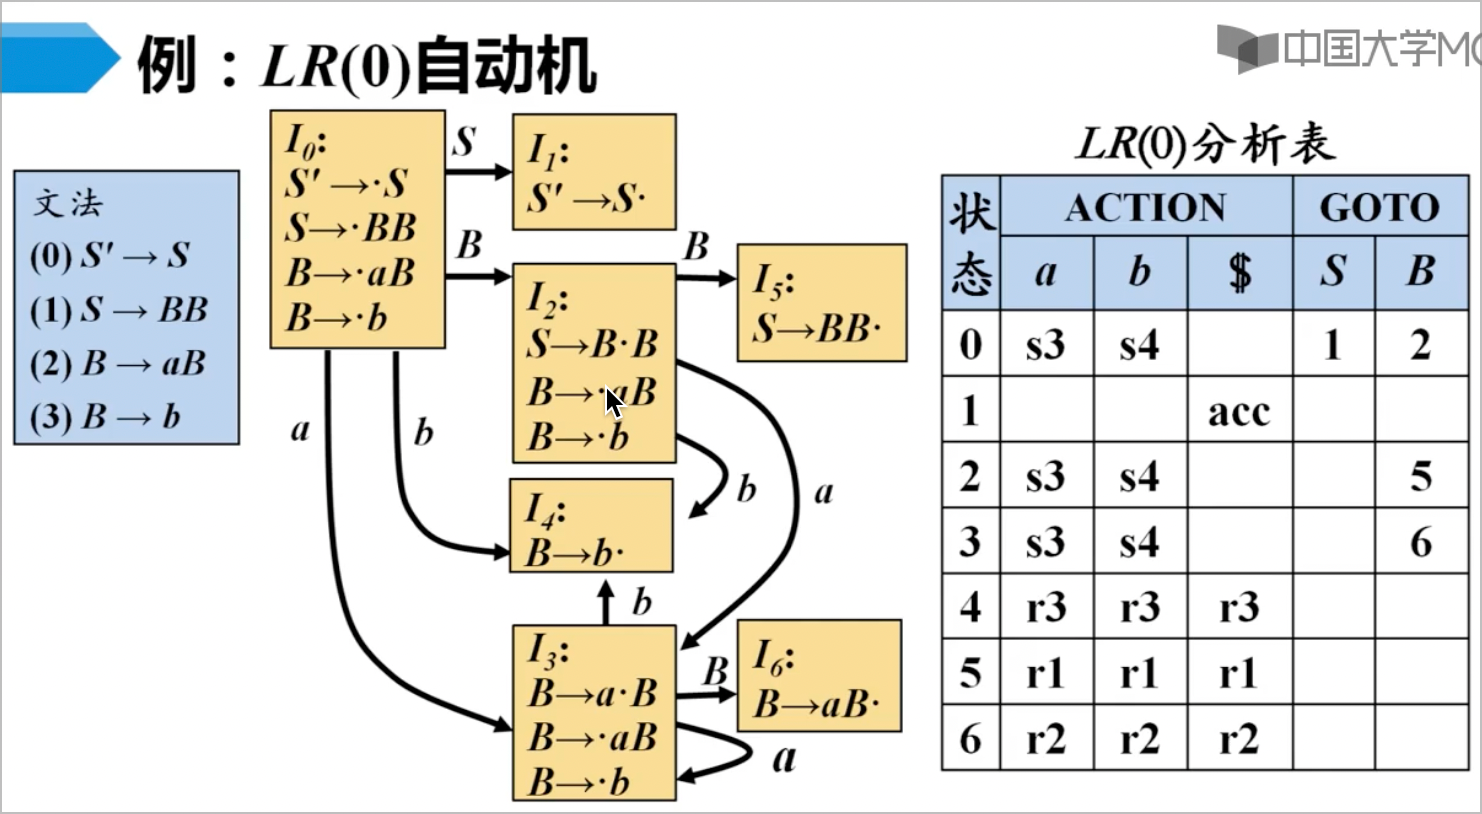
\includegraphics[width=\textwidth]{assets/LR0.png}
    \caption{LR(0)项目集}
\end{figure}

如果LR(0)分析表中没有语法分析动作冲突,那么给定的文法就称为LR(0)文法

\subsubsection{SLR分析法}

解决了部分语法分析动作冲突的问题,但是无法解决移入归约冲突(移入符$\alpha$和$FOLLOW(X)$的冲突问题)

因为SLR分析只是简单的考察了下一个输入符号b是否属于与归约项目$A\rightarrow \alpha$相关联的$FOLLOW(A)$,但$b\in FOLLOW(A)$只是归约a的一个必要条件,而非充分条件

对于产生式$A\rightarrow \alpha$的归约,在不同的使用位置,$A$会要求不同的后继符号,也就是说对于不同位置,$A$的后继符号集合应该是$FOLLOW(A)$的子集

\subsubsection{LR(1)分析法}

规范LR(1)项目:将一般形式为$[A\rightarrow \alpha\cdot\beta,a]$的项称为$LR(1)$项,其中$A\rightarrow \alpha\beta$是一个产生式,$a$是一个终结符。它表示在当前状态下,A后面要求紧跟的终结符,称为该项的展望符

\subsubsection{算符优先语法分析}

\paragraph{基本思路} 只考虑算符之间的优先关系,也就是只考虑终结符之间的优先关系

\begin{equation}
    \begin{aligned}
        G[E]:\ E & \rightarrow T|E+T|E-T \\
        T        & \rightarrow F|T*F|T/F \\
        F        & \rightarrow (E)|i
    \end{aligned}
\end{equation}

设有文法G,如果G中没有形如$A\rightarrow ...BC...$的产生式,其中B,C为\textbf{非终结符},则称G为\emph{算符文法}

设G是一个不含$\epsilon$产生式的算符文法,a和b是任意两个终结符,A,B,C是非终结符,算法优先关系$\doteq \lessdot \gtrdot $定义如下

\begin{enumerate}
    \item $a\doteq b$当且仅当G中含有形如$A\rightarrow ...ab...$或$A\rightarrow ...aBb...$的产生式
    \item $a\lessdot b$当且仅当G中含有形如$A\rightarrow ...aB...$的产生式且$B\Rightarrow^+ b...$或$B\Rightarrow^+ Cb...$,也就是说$a\lessdot FIRSTVT(B)$
    \item $a\gtrdot b$当且仅当G中含有形如$A\rightarrow ...Bb...$的产生式且$B\Rightarrow^+ ...a$或$B\Rightarrow^+ ...aC$,也就是说$LASTVT(B)\gtrdot b$
\end{enumerate}

设G是一个不含$\epsilon$产生式的算符文法,如果任一终结符对(a,b)之间\emph{至多}有$\doteq \lessdot \gtrdot $三种关系中的一种成立,则称G是一个\textbf{算符优先文法}

需要注意的是,终结符之间的优先关系是有序的,也就是说(a,b)和(b,a)是两个终结符对,允许存在$a\lessdot b,b\doteq a$同时存在

根据定义判断算符优先文法的优先级简直是神经质的,那么如何方便的做到这一点呢?

\paragraph{方法}:求解FIRSTVT集和LASTVT集

\begin{itemize}
    \item $FIRSTVT(B)=\{b|B\Rightarrow^+b... \ or\ B\Rightarrow^+ Cb...\}$
    \item $LASTVT(B)=\{a|B\Rightarrow^+...a \ or\ B\Rightarrow^+ ...aC\}$
\end{itemize}

构造规则如下

\begin{itemize}
    \item FIRSTVT
          \begin{enumerate}
              \item 若有$T\rightarrow a...$或$T\rightarrow Ra...$,则$a\in FIRSTVT(T)$
              \item 若有$a\in FIRSTVT(R)$且有产生式$T\rightarrow R...$,则$a\in FIRSTVT(T)$
              \item 迭代
          \end{enumerate}
    \item LASTVT
          \begin{enumerate}
              \item 若有$T\rightarrow ...a$或$T\rightarrow ...aR$,则$a\in LASTVT(T)$
              \item 若有$a\in LASTVT(R)$且有产生式$T\rightarrow ...R$,则$a\in LASTVT(T)$
              \item 迭代
          \end{enumerate}
\end{itemize}

举例文法

\begin{equation}
    \begin{aligned}
        E & \rightarrow E+T|T \\
        T & \rightarrow T*F|F \\
        F & \rightarrow (E)|i
    \end{aligned}
\end{equation}

\begin{table}[H]
    \centering
    \begin{tabular}{|p{2cm}<{\centering}|p{1cm}<{\centering}|p{1cm}<{\centering}|p{1cm}<{\centering}|p{1cm}<{\centering}|p{1cm}<{\centering}|}
        \hline
        F & + & * & ( & ) & i \\
        \hline
        E & 1 & 1 & 1 &   & 1 \\
        T &   & 1 & 1 &   & 1 \\
        F &   &   & 1 &   & 1
    \end{tabular}
\end{table}

\begin{table}[H]
    \centering
    \begin{tabular}{|p{2cm}<{\centering}|p{1cm}<{\centering}|p{1cm}<{\centering}|p{1cm}<{\centering}|p{1cm}<{\centering}|p{1cm}<{\centering}|}
        \hline
        L & + & * & ( & ) & i \\
        \hline
        E & 1 & 1 &   & 1 & 1 \\
        T &   & 1 &   & 1 & 1 \\
        F &   &   &   & 1 & 1
    \end{tabular}
\end{table}

\begin{table}[H]
    \centering
    \begin{tabular}{|p{3cm}<{\centering}|p{1cm}<{\centering}|p{1cm}<{\centering}|p{1cm}<{\centering}|p{1cm}<{\centering}|p{1cm}<{\centering}|}
        \hline
        算符优先分析表 & +          & *          & (          & )         & i          \\
        \hline
        +       & $\gtrdot$  & $\lessdot$ & $\lessdot$ & $\gtrdot$ & $\lessdot$ \\
        \hline
        *       & $\gtrdot$  & $\gtrdot$  & $\lessdot$ & $\gtrdot$ & $\lessdot$ \\
        \hline
        (       & $\lessdot$ & $\lessdot$ & $\lessdot$ & $\doteq$  & $\lessdot$ \\
        \hline
        )       & $\gtrdot$  & $\gtrdot$  &            & $\gtrdot$ &            \\
        \hline
        i       & $\gtrdot$  & $\gtrdot$  &            & $\gtrdot$ &            \\
        \hline
    \end{tabular}
\end{table}

\begin{equation}
    \begin{aligned}
        G[S]:\ S & \rightarrow S;G|G  \\
        G        & \rightarrow G(T)|H \\
        H        & \rightarrow a|(S)  \\
        T        & \rightarrow T+S|S
    \end{aligned}
\end{equation}

给出上述符号串\textbf{a;(a+a)}的算符优先分析过程。

\begin{table}[H]
    \centering
    \begin{tabular}{|p{2cm}<{\centering}|p{1cm}<{\centering}|p{1cm}<{\centering}|p{1cm}<{\centering}|p{1cm}<{\centering}|p{1cm}<{\centering}|}
        \hline
        F & ; & ( & ) & a & + \\
        \hline
        S & 1 & 1 &   & 1 &   \\
        G &   & 1 &   & 1 &   \\
        H &   & 1 &   & 1 &   \\
        T & 1 & 1 &   & 1 & 1
    \end{tabular}
\end{table}

\begin{table}[H]
    \centering
    \begin{tabular}{|p{2cm}<{\centering}|p{1cm}<{\centering}|p{1cm}<{\centering}|p{1cm}<{\centering}|p{1cm}<{\centering}|p{1cm}<{\centering}|}
        \hline
        L & ; & ( & ) & a & + \\
        \hline
        S & 1 &   & 1 & 1 &   \\
        G &   &   & 1 & 1 &   \\
        H &   &   & 1 & 1 &   \\
        T & 1 &   & 1 & 1 & 1
    \end{tabular}
\end{table}

\begin{table}[H]
    \centering
    \begin{tabular}{|p{3cm}<{\centering}|p{1cm}<{\centering}|p{1cm}<{\centering}|p{1cm}<{\centering}|p{1cm}<{\centering}|p{1cm}<{\centering}|}
        \hline
        算符优先表 & ;          & (          & )         & a          & +          \\
        \hline
        ;     & $\gtrdot$  & $\lessdot$ & $\gtrdot$ & $\lessdot$ & $\gtrdot$  \\
        \hline
        (     & $\lessdot$ & $\lessdot$ & $\doteq$  & $\lessdot$ & $\lessdot$ \\
        \hline
        )     & $\gtrdot$  & $\gtrdot$  & $\gtrdot$ & err        & $\gtrdot$  \\
        \hline
        a     & $\gtrdot$  & $\gtrdot$  & $\gtrdot$ & err        & $\gtrdot$  \\
        \hline
        +     & $\lessdot$ & $\lessdot$ & $\gtrdot$ & $\lessdot$ & $\gtrdot$  \\
        \hline
    \end{tabular}
\end{table}

\begin{table}[H]
    \centering
    \begin{tabular}{|p{3cm}<{\centering}|p{2cm}<{\centering}|p{3cm}<{\centering}|p{2cm}<{\centering}|}
        \hline
        栈        & 当前输入符 & 输入串剩余部分  & 下一步动作 \\
        \#       & a     & ;(a+a)\# & 移入    \\
        \#a      & ;     & (a+a)\#  & 归约    \\
        \#T      & ;     & (a+a)\#  & 移入    \\
        \#T;     & (     & a+a)\#   & 移入    \\
        \#T;(    & a     & +a)\#    & 移入    \\
        \#T;(a   & +     & a)\#     & 归约    \\
        \#T;(T   & +     & a)\#     & 移入    \\
        \#T;(T+  & a     & )\#      & 移入    \\
        \#T;(T+a & )     & \#       & 归约    \\
        \#T;(T+T & )     & \#       & 归约    \\
        \#T;(T   & )     & \#       & 移入    \\
        \#T;(T)  & \#    &          & 归约    \\
        \#T;T    & \#    &          & 归约    \\
        \#T      & \#    &          & 移入    \\
        \#T\#    &       &          & 结束    \\
    \end{tabular}
\end{table}

\section{语法制导翻译}

\begin{figure}[H]
    \centering
    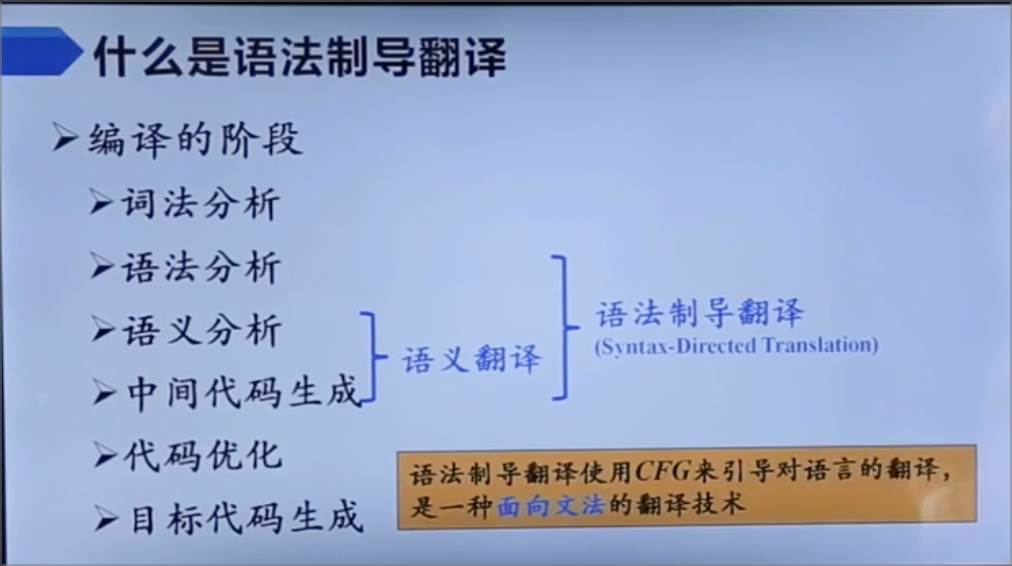
\includegraphics[width=\textwidth]{assets/语法制导翻译概念.png}
    \caption{语法制导翻译}
\end{figure}

\paragraph{如何表示语义信息} 给CFG中的文法符号设置语义属性,用来表示语法成分对应的语义信息(比如说变量类型、值、存放地址等等)

\paragraph{如何计算语义属性} 对于给定的输入串x,构建x的语法分析树,并利用与产生式(语法规则)相关联的语义规则来计算分析树中各节点的语义属性值

\subsection{语法制导定义SDD}

SDD是对CFG的拓展,它将每个文法符号和一个语义属性集合相关联,将每个产生式和一组语义规则相关联,这些规则用于计算该产生式中各文法符号的属性值

如果X是一个文法符号,a是X的一个属性,那么$X.a$表示X的属性a在某个标号为X的分析树节点上的值

文法符号的属性种类
\begin{itemize}
    \item 综合属性:在分析树节点N上的非终结符A的综合属性只能通过N的子节点本身的属性值来定义
    \item 继承属性:在分析树节点N上的非终结符A的继承属性只能通过N的父节点、N的兄弟节点、N本身的属性值来定义
\end{itemize}

\begin{equation}
    \begin{aligned}
        E\rightarrow E_1+T  \\
        E.val=E_1.val+T.val \\
        D\rightarrow TL     \\
        L.inh=T.type
    \end{aligned}
\end{equation}

\subsection{语法制导翻译SDT}

\paragraph{概念} SDT是在产生式右部嵌入了程序片段的CFG,这些程序片段称为语义动作。按照惯例,语义动作写在产生式右部的花括号中

\begin{equation}
    \begin{aligned}
        D\rightarrow T\{L.inh=T.type\} L
    \end{aligned}
\end{equation}

这里的含义是,当分析出终结符T的时候,就可以把T的属性值赋给L的inh属性

\section{中间代码生成}

\subsection{活动记录}

一个典型的活动记录可以分为三部分:

\begin{enumerate}
    \item 局部数据区:存放模块中定义的各个\textbf{局部变量}
    \item 参数区:存放\emph{隐式参数}和\emph{显式参数(形参数据区)}
          \begin{itemize}
              \item prev abp: 存放调用模块记录基地址
              \item ret addr: 返回地址
              \item ret value: 函数返回值
          \end{itemize}
    \item display区:\textbf{存放各外层模块活动记录的基地址}
\end{enumerate}

\end{document}